\documentclass{report}
\usepackage[francais]{babel}
\usepackage[utf8]{inputenc}
\usepackage[T1]{fontenc}
\usepackage{fontspec}

\title{Projet NTR : Routage opportuniste}
\author{Rogala Jimmy, de la Ferté Apolline, Dubois Quentin, Gachelin Jérémie}
\date{}

\begin{document}
\maketitle


\chapter{Contexte}

\paragraph{Ce projet concerne l'approfondissement de l'étude des protocoles de 
routage opportuniste dans les réseaux sans fil. Il s'agit de simuler ces nouveaux protocoles "opportunistes" adaptés au milieu sans fil, pour choisir le meilleur chemin en fonction des nombreuses contraintes de cet environnement.}

\paragraph{Les contraintes à prendre en compte, en complément des métriques habituelles pour tous les environnements comme le nombre de saut et le coût, sont les différentes conditions radio influant grandement sur les transmissions.}

\paragraph{L'objectif visé est d'obtenir, en autres, une augmentation du débit global du système, une économie d'énergie et une amélioration de la QoS (Qualité de Service).}

\chapter{Hypothèses techniques}

\paragraph{Dans un choix de simplicité, nous avons utilisé le langage Java, nous permettant de travailler facilement sur nos différents systèmes d'exploitation. C'est de plus un langage dont nous possédions tous les bases.}

\paragraph{Le programme simule un réseau qui est constitué d'une grille de noeuds. Il est structuré de façon à rendre la communication entre les noeuds plus aisée. Chaque noeud représente un appareil (Device) et est relié à d'autres noeuds via des liens (Link). Chaque lien possède différentes caractéristiques de débits : débit instantané, moyen, minimum et maximum, générés aléatoirement pour chaque lien et modifiables à souhait.}

\paragraph{Les unités utilisées dans le cadre de notre simulation, tant en terme de débit que de temps, sont totalement fictives et ne se réfèrent à aucune unité de base du Système international.}

\chapter{Scénario}

\paragraph{Nous avons simulé la transmission de données depuis un point A, l'expéditeur, jusqu'à un point B, le destinataire. Chaque noeud possédant une file d'attente de paquets à transmettre. La transmission se fait à chaque unité de temps, la quantité de données envoyée dépend du noeud destinataire ainsi que du débit du lien qui les relie. Le noeud destinataire est fourni à chaque noeud en fonction de l'algorithme de routage utilisé.}

\paragraph{La simulation se termine lorsque le noeud d'arrivé a reçu l'ensemble des données transmises par le noeud de départ. Nous pouvons donc obtenir, pour un réseau donné et une quantité de paquets, un nombre d'unité de temps représentant la performance des différents algorithmes.}

\paragraph{}

\chapter{Résultats analysés}

\begin{center}
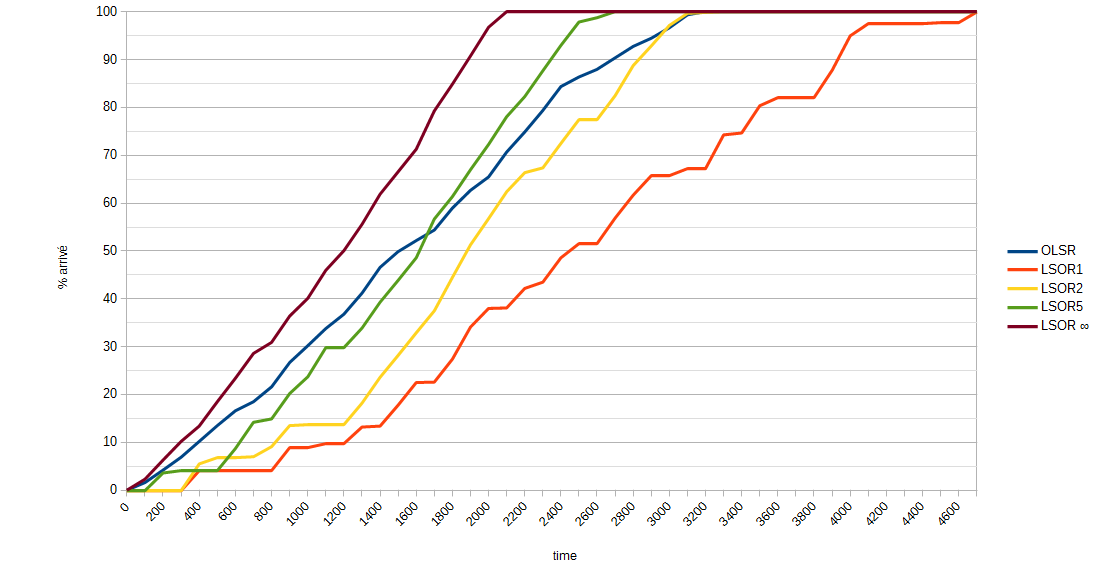
\includegraphics[scale=0.4]{quentin_result/courbes.png}
\end{center}

\paragraph{}

\chapter{Conclusion}

\paragraph{}
\end{document}
